\chapter{Question 4}
\label{available-representation}

\textbf{Use MDS to create a JPEG of the blogs similar to slide 29. How many iterations were required?}\\\\

Following are the steps I have taken to solve the problem:

\begin{itemize}
\item I imported the `clusters.py' mentioned in `question 2' and used the code described in `presentation slide 29' to create a JPEG of the most similar blogs using MDS. This code is in Listing \ref{lst:q4code1} 
\newpage
\item The output JPEG file is illustrated in \ref{fig:q4fig1}. 
\begin{figure}[h!]
\begin{center}
\hspace*{-3cm} 
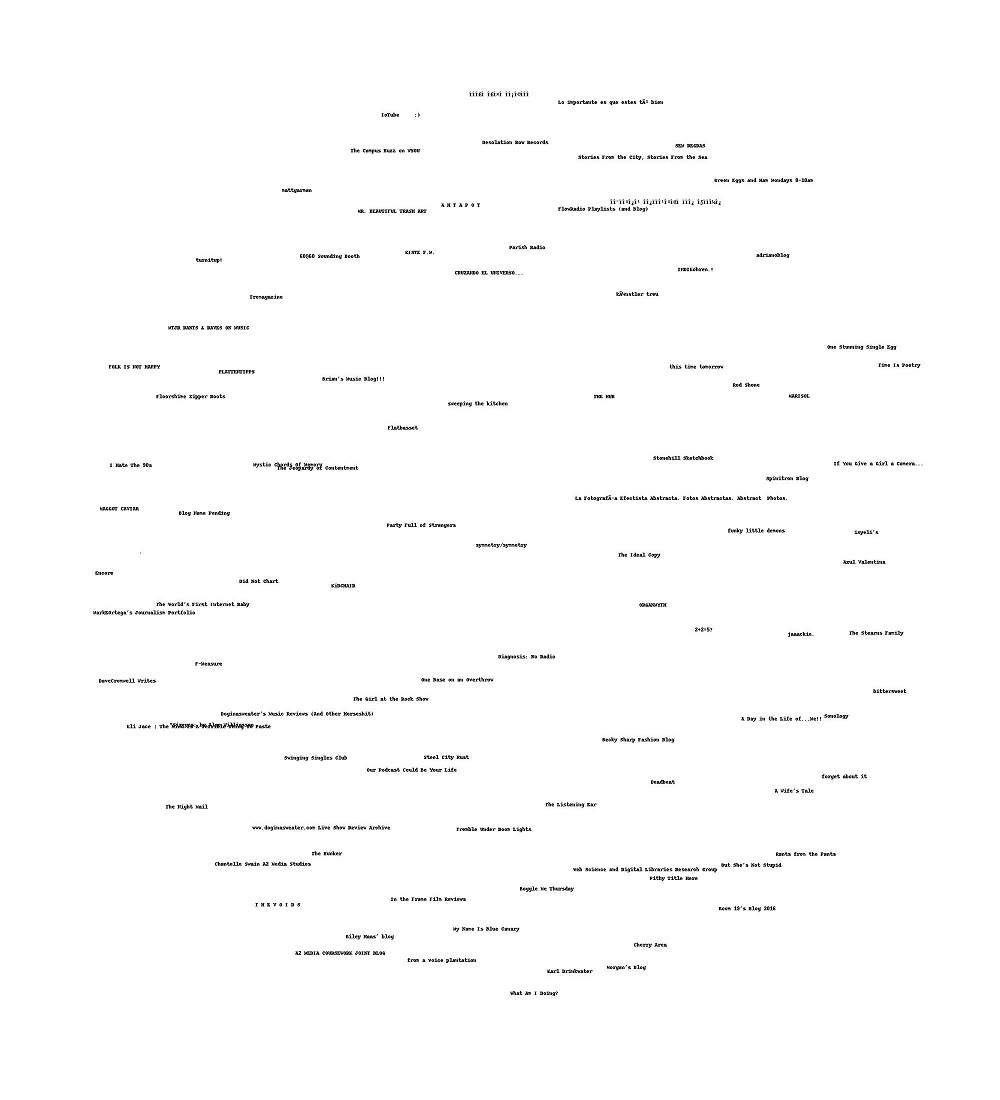
\includegraphics[scale=0.55, keepaspectratio=true]{figures/blogs2d.jpg}
\caption{JPEG of blogs using MDS}
\label{fig:q4fig1}
\end{center}
\end{figure}
\item To get the number of iterations I have written a print statement in function `scaledown(data,distance=pearson,rate=0.01)' of `clusters.py'. `304'  iterations were required for creating the JPEG using MDS. The file `numberOfIterations.txt' has `total error' and `iteration count'.
\item The python code `clusters.py' that I downloaded from the PCI book is illustrated in Listing \ref{lst:q4code2}
\end{itemize}


\textbf{Code Listing}
\sloppy
\lstinputlisting[language=Python,caption=Python code for creating MDS,frame=single,breaklines=true,label=lst:q4code1, tabsize=2, captionpos=b,numbers=left,showspaces=false,showstringspaces=false,basicstyle=\footnotesize]{src/createMDS.py}


\textbf{Code Listing}
\sloppy
\lstinputlisting[language=Python,caption=Python code `clusters.py' from PCI ,frame=single,breaklines=true,label=lst:q4code2, tabsize=2, captionpos=b,numbers=left,showspaces=false,showstringspaces=false,basicstyle=\footnotesize]{src/clusters.py}